\chapter{Implementazione}
\label{implementazione}

\section{Modalità di computazione}
\label{computationMode}
\subsection{Low Computation mode}

\subsection{High Computation mode}

\subsection{Testing Computation mode}
\label{tcm}


\section{Canali di comunicazione}

\subsection{I2C}
\label{imp_i2c}
Per la comunicazione tra l' \textbf{IMU} e il \textbf{Microcontrollore}, si è utilizzato un canale di comunicazione seriale bifilare noto come \textit{Inter Integrated Circuit}, abbreviato \textbf{I2C}, come mostrato dalla seguente figura:
\begin{figure}[H]  
	\centering 
	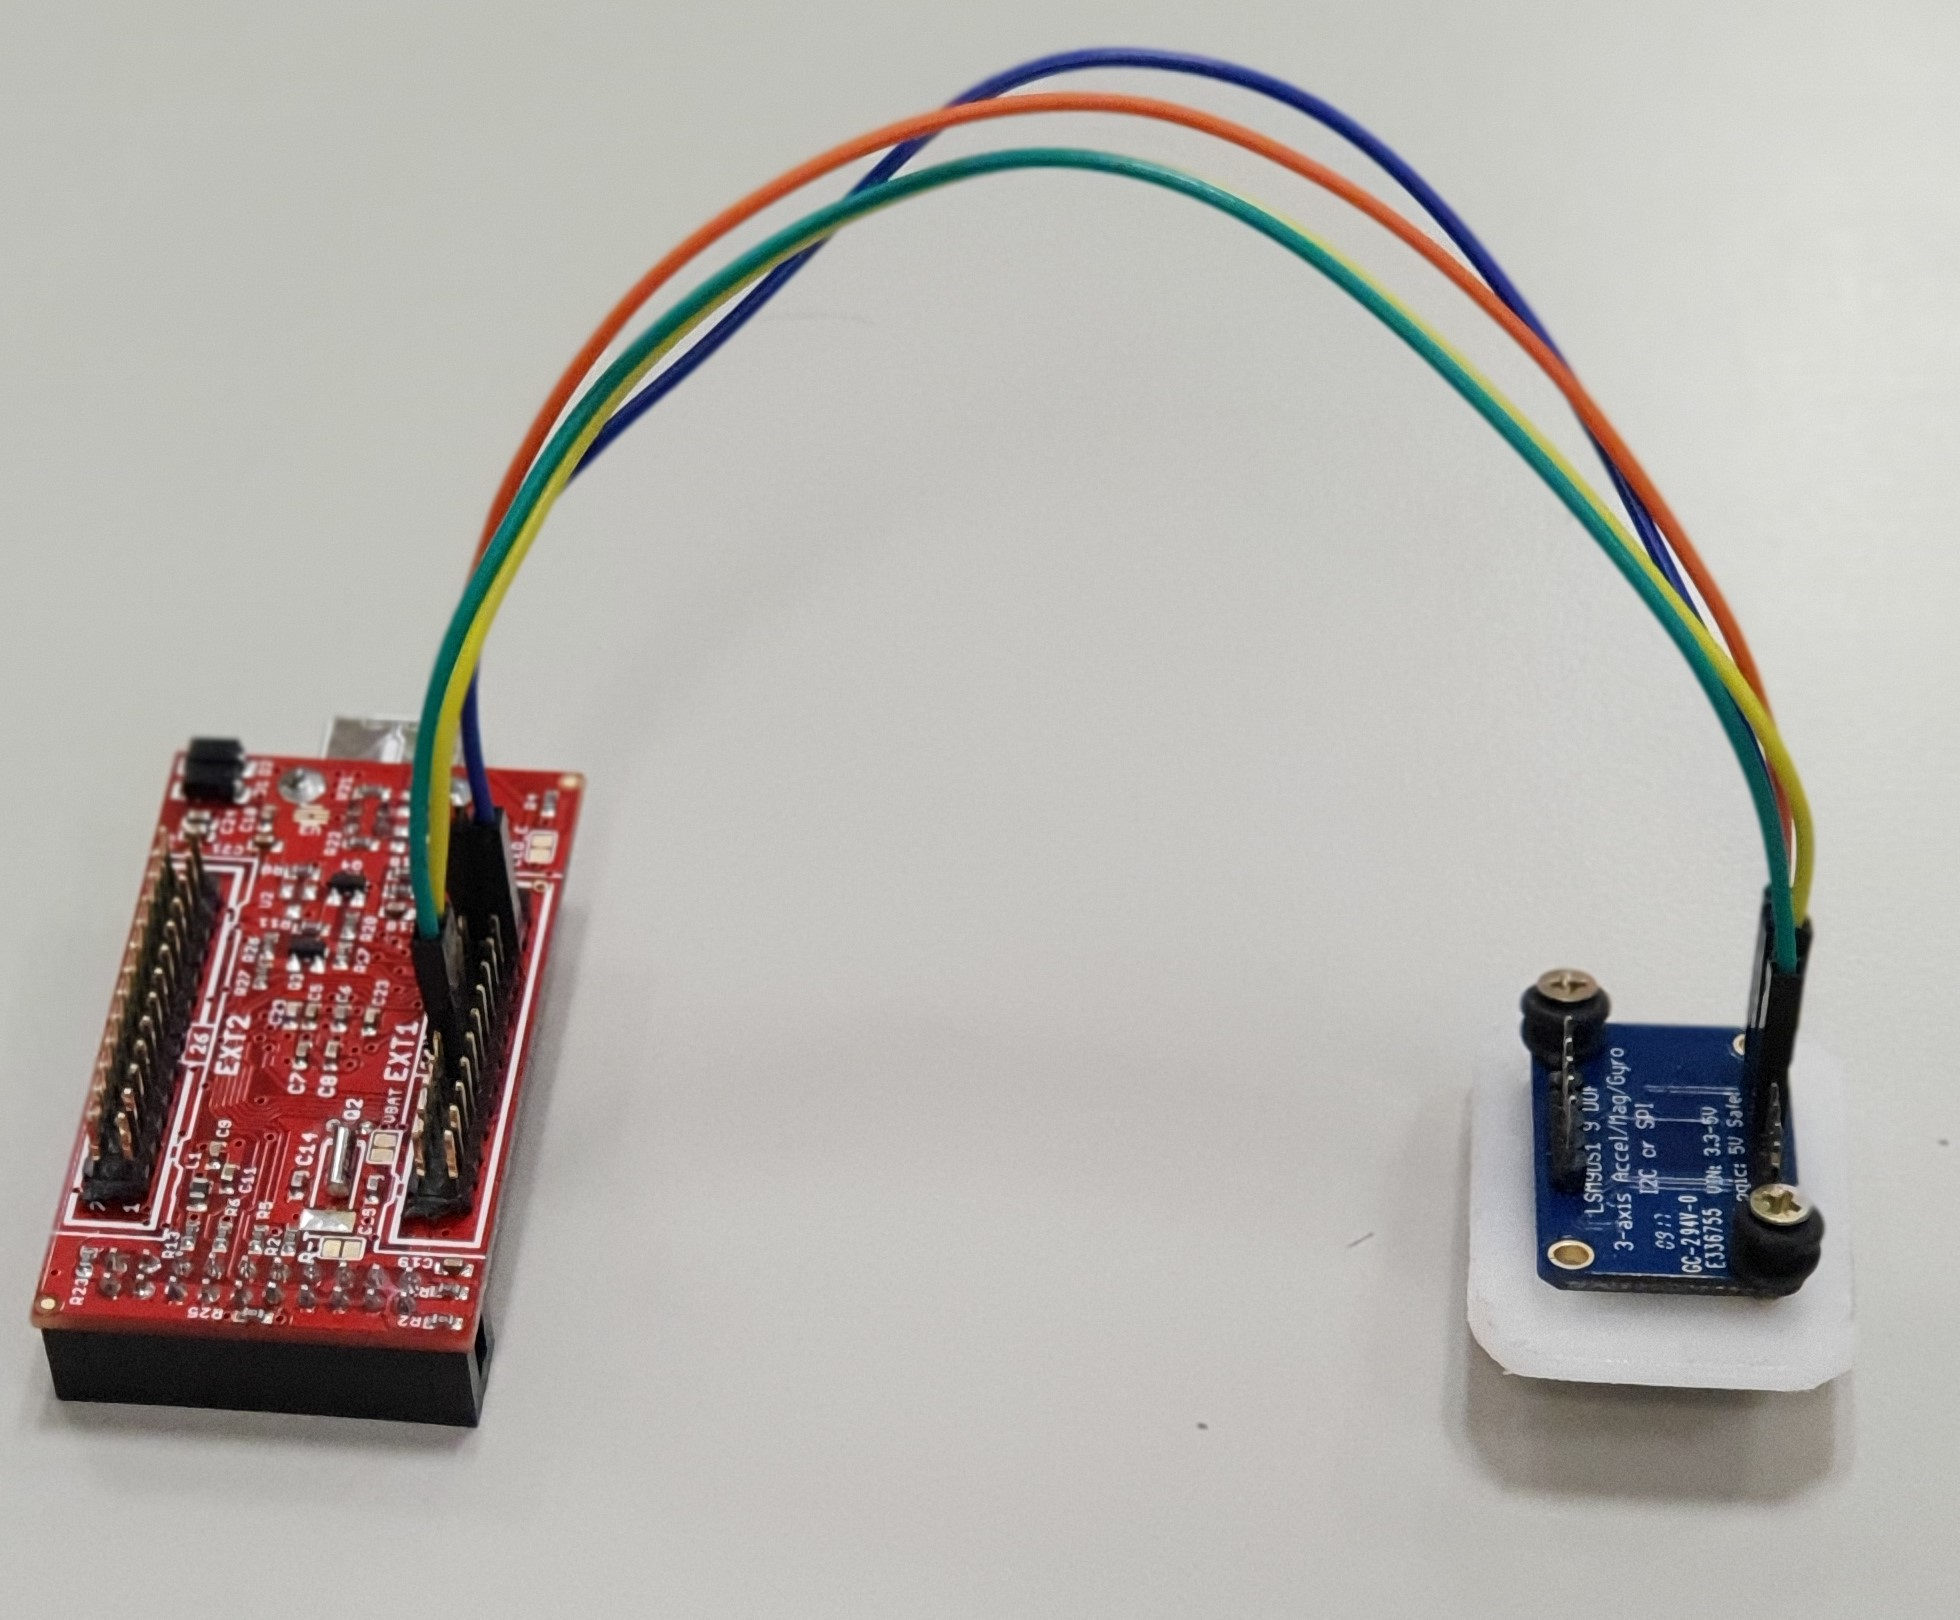
\includegraphics[scale=0.1]{implementazione/i2cFoto.jpg}
	\caption{Foto del canale di comunicazione I2C tra il microcontrollore e l'unità di misura inerziale.}
	\label{fig:i2cFoto}
\end{figure}
Il protocollo \cite{i2cWiki} dell'I2C richiede due linee seriali per comunicare correttamente:
\begin{itemize}
\item SDA (\textit{Serial Data}) per i dati
\item SCL (\textit{Serial Clock}) per sincronizzare i dispositivi
\end{itemize}
Vanno inoltre aggiunte una connessione di riferimento alla massa e una alla linea di alimentazione (tipicamente 5 o 3,3 V) a cui sono connessi resistori di \textit{pull-up}, come mostrato dalla figura seguente:
\begin{figure}[H]  
	\centering 
	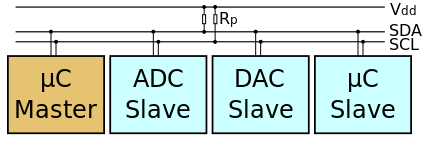
\includegraphics[scale=0.6]{implementazione/i2c.png}
	\caption{Rappresentazione di dispositivi collegati mediante I2C}
	\label{fig:i2c}
\end{figure}
L'I2C utilizza un indirizzo a 7 bit per un totale di 128 indirizzi disponibili. Poiché di questi 16 sono riservati, si ha un totale finale di 112 dispositivi collegabili alla medesima linea.\\
La velocità è il grande limite di questa comunicazione, infatti con le recenti revisioni si è riuscita a raggiungere una velocità massima di 3,4 Mbit/s (detto anche \textit{High Speed Mode}). Nello specifico di questa tesi lo si è utilizzato in \textit{fast mode} che corrisponde ad una velocità di 400 Kbit/s.\\
I dispositivi collegati al bus possono essere di due tipi:
\begin{itemize}
\item Un \textit{Master} che controlla la SCL, inizializza le comunicazioni e invia dati
\item Uno o più \textit{Slave} che rispondono ad un master e inviano dati
\end{itemize}

Il messaggio viene spezzato in due parti:
	\begin{itemize}
		\item \textit{Address frame} dove il \textit{master} indica l'indirizzo dello \textit{slave} interessato alla comunicazione
		\item uno o più \textit{Data frames} contenenti l'informazione da trasmettere
	\end{itemize}
I dati sono "piazzati" sulla linea SDA dopo che la linea SCL è posta a zero dal master, questi dati verranno letti dal dispositivo specificato nell'\textit{address frame} quando il \textit{master} riporterà la linea SCL al valore alto.\\
Relativamente al lavoro di questa tesi si identificano il \textit{Microcontrollore} come \textit{master} mentre l'\textit{IMU} come \textit{slave}. Nello specifico la comunicazione consiste nella lettura periodica da parte del microcontrollore dei valori misurati dai sensori all'interno dell'IMU. Tale lettura è stata realizzata leggendo i singoli registri ad 8 bit dei sensori (per maggiori dettagli si veda la stima temporale in sez.\ref{analisiTemporale}) attraverso lo script in Appendice \ref{scriptXLGRead} e rappresentato dalla seguente figura:
\begin{figure}[H]  
	\centering 
	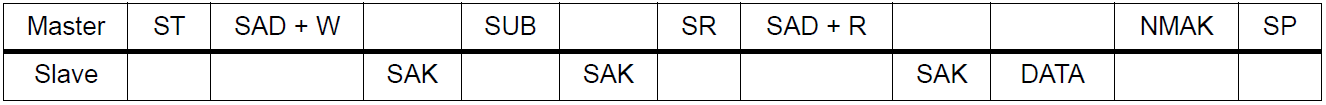
\includegraphics[scale=0.5]{implementazione/i2cRead.png}
	\caption{Rappresentazione del flusso di dati generato per la lettura, tramite I2C, di un registro ad 8 bit.}
	\label{fig:i2cRead}
\end{figure}
 Dove:
 \begin{itemize}
	\item  \textit{ST} è il segnale di inizio di una comunicazione
	\item \textit{SAD + W} include l'indirizzo del dispositivo slave mentre l'ultimo bit specifica che il master sta per scrivere
	\item \textit{SAK} lo slave con l'indirizzo specificato precedentemente risponde con un segnale di \textit{acknowledge}
	\item \textit{SUB} è l'indirizzo del registro interno del dispositivo specificato precedentemente
	\item \textit{SAK} lo slave risponde con un segnali di \textit{acknowledge} se l'indirizzo del registro esiste
	\item \textit{SR} è il bit di ripetizione dello start utilizzato in combinazione con SAD+R/W
	\item \textit{SAD + R} include l'indirizzo del dispositivo slave mentre l'ultimo bit specifica che il master vuole ricevere dati
	\item \textit{SAK} segnale di \textit{acknowledge} da parte dello \textit{slave}
	\item \textit{DATA} dati trasmetti nel formato ad 8 bit
	\item \textit{NMAK} segnale di  \textit{non acknowledge} da parte del \textit{master}
	\item \textit{SP} bit di stop della comunicazione
\end{itemize}
Tuttavia questa lettura non è sempre la migliore, infatti è possibile continuare a leggere i registri interni dello \textit{slave} trasmettendo il segnale di \textit{MAK} invece del segnale di \textit{NMAK} mostrato in Fig.\ref{fig:i2cRead}. In questo modo l'IMU incrementerà l'indirizzo del registro interno di partenza specificato in \textit{SUB} e provvederà a trasmettere il valore del registro interno successivo ad esso. Questa funzionalità è molto utile quando si devono leggere dati, come in questo caso, che sono rappresentati con più registri. Così facendo infatti si riduce l'\textit{overhead} della trasmissione e si migliora quindi il goodput generale rispetto alla lettura ripetuta dei singoli registri.\\

 
	
\subsection{USB CDC}
\label{imp_usbcdc}
Per la comunicazione tra il \textit{microcontrollore} e l'elaboratore si è utilizzato un canale di comunicazione USB nella classe CDC \cite{usbCDC}, mostrato in Fig.\ref{usbFoto}, attraverso la libreria \textit{HAL} \cite{hal} fornita da \textit{STM}.
\begin{figure}[H]  
	\centering 
	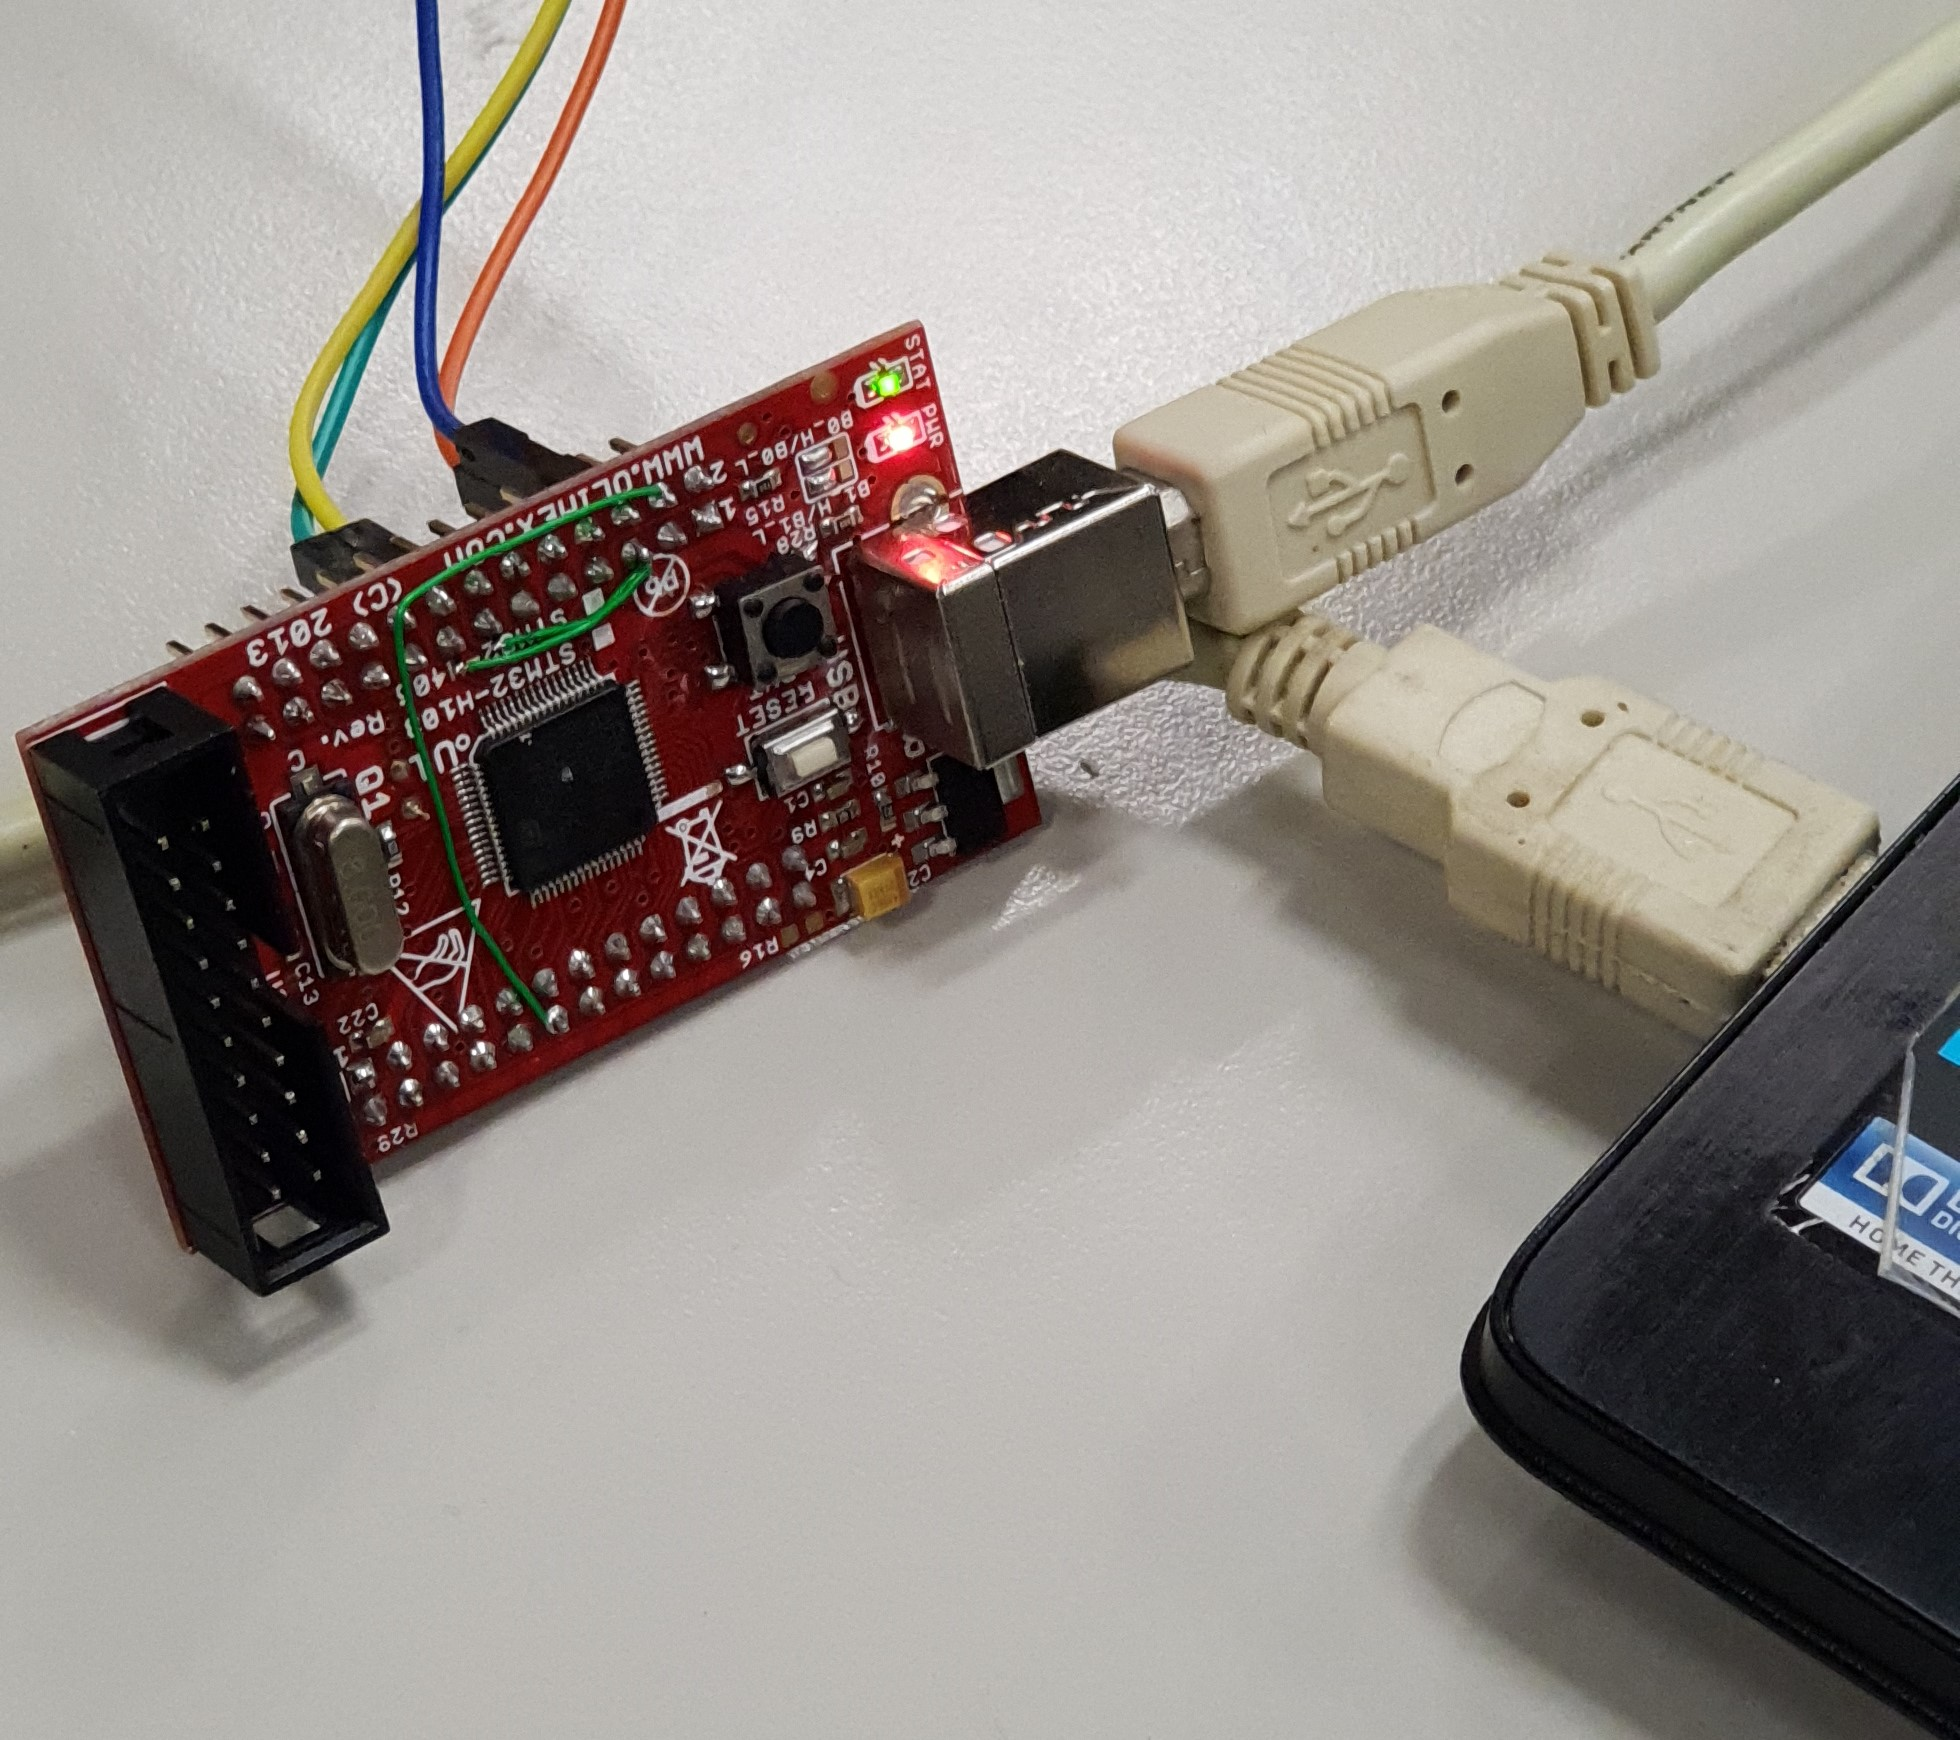
\includegraphics[scale=0.1]{implementazione/usbFoto.jpg}
	\caption{Foto del canale di comunicazione USB usato nella classe CDC per la trasmissione dei dati dal microcontrollore all'elaboratore.}
	\label{fig:usbFoto}
\end{figure}
Un dispositivo CDC è composto \cite{usbCDC2} dalle seguenti interfacce:
\begin{itemize}
	\item \textit{Communications Class Interface} (CCI)
	\item \textit{Data Class Interface} (DCI)
\end{itemize}
L'interfaccia CCI è responsabile della gestione del dispositivo e in alcuni casi anche della gestione delle chiamate. Per gestione del dispositivo si intendono le configurazioni necessarie da eseguire sul \textit{device} e la notifica degli eventi, mentre per gestione della chiamata si intendono le operazioni necessarie per stabilire e terminare una comunicazione. La CCI è obbligatoria per tutti i dispositivi CDC in quanto lo identifica specificando il modello di comunicazione supportato dal dispositivo stesso.\\
L'interfaccia DCI è responsabile della trasmissione dei dati, infatti i dati trasmessi e/o ricevuti non seguono uno specifico formato. Tutte le interfacce di questo tipo possono essere viste come interfacce subordinate della CCI.\\
Tutti i dispositivi CDC devono avere almeno un'interfaccia CCI e zero o più interfacce DCI. Un CCI e ogni suo DCI subordinato forniscono una specifica funzionalità al dispositivo.\\
In generale un \textit{device} CDC potrebbe supportare diverse funzionalità e quindi essere composto da diversi set di CCI e DCI, come mostrato dalla figura seguente:
\begin{figure}[H]  
	\centering 
	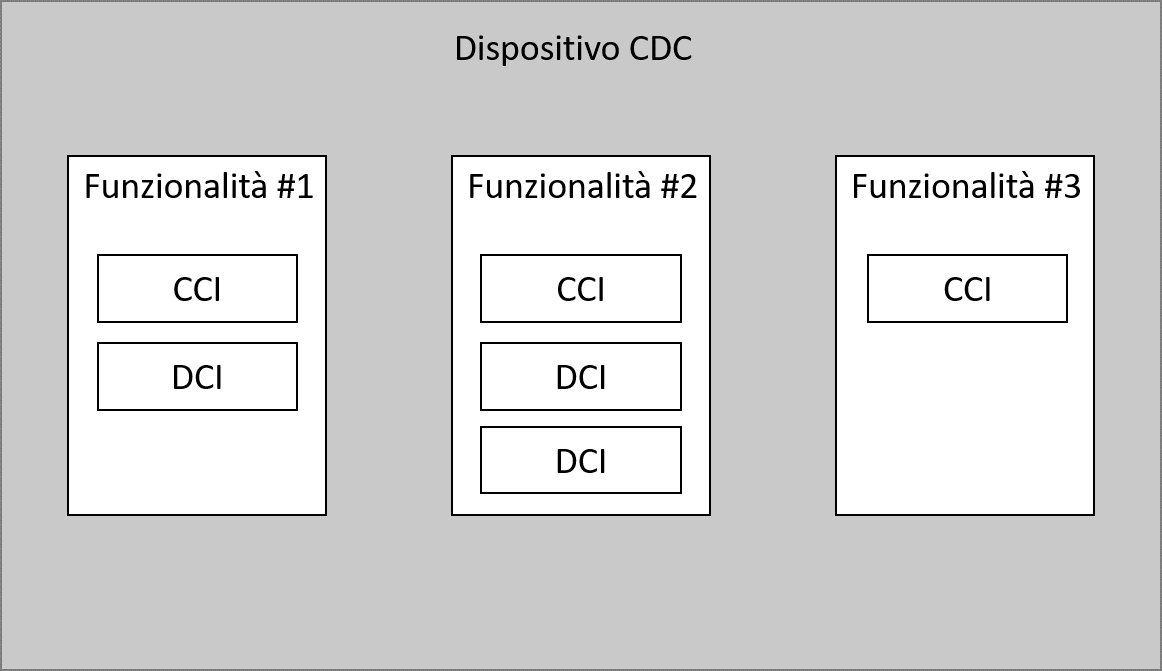
\includegraphics[scale=0.4]{implementazione/cdcDevice.png}
	\caption{Rappresentazione di un dispositivo CDC che supporta tre diverse funzionalità.}
	\label{fig:cdcDevice}
\end{figure}
Un dispositivo CDC solitamente usa le senguenti combinazioni di \textit{endpoints}:
\begin{itemize}
	\item Una coppia di \textit{endpoints} di controllo IN e OUT chiamate \textit{endpoint di default}.
	\item Un \textit{endpoint} opzionale chiamato \textit{bulk} o \textit{interrupt IN}
	\item Una coppia di \textit{bulk} o \textit{endpoints} IN e OUT asincroni
\end{itemize}
La tabella \ref{tab:endpoints} mostra gli usi dei differenti \textit{endpoints} sopracitati e da quale interfaccia sono utilizzati.
\begin{table}[H]
	\centering
	\label{tab:endpoints}
	\begin{tabular}{|c|c|c|c|}
		\hline
		\textbf{Endpoint}                          & \multicolumn{1}{l|}{\textbf{Direzione}}        & \multicolumn{1}{l|}{\textbf{Interfaccia}} & \textbf{Uso}                                                                                                                                                                   \\ \hline
		Control IN                                 & Device-\textgreater{}Host                      & CCI                                       & \begin{tabular}[c]{@{}c@{}}Richiesta standard \\ per l'enumerazione,\\ richiesta specifica della classe,\\ controllo del dispositivo e\\ controllo della chiamata\end{tabular} \\ \hline
		Control OUT                                & Host-\textgreater{}Device                      & CCI                                       & "..."                                                                                                                                                                          \\ \hline
		Interrupt o bulk IN                        & Device-\textgreater{}Host                      & CCI                                       & \begin{tabular}[c]{@{}c@{}}Notifica di un evento\\ come lo stato della linea \\ o della rete\end{tabular}                                                                      \\ \hline
		\multicolumn{1}{|l|}{Bulk o OUT asincrono} & \multicolumn{1}{l|}{Host-\textgreater{}Device} & DCI                                       & \begin{tabular}[c]{@{}c@{}}Comunicazione di \\ dati grezzi o formattati\end{tabular}                                                                                           \\ \hline
		Bulk o IN asincrono                        & Host-\textgreater{}Device                      & DCI                                       & "..."                                                                                                                                                                          \\ \hline
	\end{tabular}
	\caption{Tabella con gli usi tipici degli \textit{endpoints} per comunicazioni USB-CDC}
\end{table}
La libreria HAL utilizzata nel lavoro di questa tesi, utilizza due tipi di \textit{endpoints} per la comunicazione:
\begin{itemize}
	\item \textit{Endpoint Bulk} per il trasferimento dei dati (1 \textit{endpoint} di OUT e 1 \textit{endpoint} di IN)
	\item \textit{Endpoint interrupt} per il controllo della comunicazione (richieste CDC, 1 \textit{endpoint} IN)
\end{itemize}
Il trasferimento dei dati IN (dal \textit{device} verso l'\textit{host}) è gestito periodicamente in base alle richieste dell'\textit{host} (il \textit{device} specifica l'intervallo di tempo tra le richieste dei pacchetti). Per questo motivo, un buffer statico circolare viene usato per memorizzare i dati mandati dal terminale del \textit{device} (esempio USART nel caso di una \textit{Virtual COM Port}).\\
In generale, la comunicazione USB è molto più veloce dell'output del terminale (ad esempio il bitrate massimo di un USART è tipicamente 115 Knps mentre il bitrate dell'USB 1.1 è 12 Mbps in \textit{Full speed mode} o 480 Mbps in \textit{High speed mode}). Di conseguenza, prima di mandare nuovi pacchetti l'\textit{host} deve aspettare finché il \textit{device} non termina di processare i dati precedentemente inviati. Quindi, nel caso di data OUT dall'\textit{host} verso il \textit{device} l'uso di un buffer statico circolare non avrebbe senso. Il driver sul \textit{device} aspetta che la procedura di processamento del dato precedente sia terminata prima di mandare un segnale di \textit{acknowledge} all'\textit{host}. \\
Infine la gestione delle richieste di controllo viene effettuata utilizzando o un \textit{endpoint} pari a zero oppure attraverso un \textit{endpoint interrupt} infatti se la dimensione del pacchetto di richiesta non eccede i 64 bytes, allora l'\textit{endpoint 0} è sufficiente a gestire tale richiesta. 
